\documentclass[11pt]{beamer}

% This file is a solution template for:

% - Talk at a conference/colloquium.
% - Talk length is about 20min.
% - Style is ornate.

% Copyright 2004 by Till Tantau <tantau@users.sourceforge.net>.
%
% In principle, this file can be redistributed and/or modified under
% the terms of the GNU Public License, version 2.
%
% However, this file is supposed to be a template to be modified
% for your own needs. For this reason, if you use this file as a
% template and not specifically distribute it as part of a another
% package/program, I grant the extra permission to freely copy and
% modify this file as you see fit and even to delete this copyright
% notice.


\mode<presentation>
{
  \usetheme{Warsaw}
  % or ...

  % \setbeamercovered{transparent}
  % or whatever (possibly just delete it)
}


\usepackage[icelandic]{babel}
% or whatever
\selectlanguage{icelandic}

\usepackage[latin1]{inputenc}
% or whatever

\usepackage{times}
\usepackage[T1]{fontenc}
\usepackage{float}
\usepackage{amssymb}
\usepackage[normalem]{ulem}
\usepackage{booktabs}
\usepackage{multirow}

\newcommand{\perm}{{\mathfrak S}}
\newcommand{\clpreim}{\texttt{ClassicalPreim}}
\newcommand{\meshpreim}{\texttt{MeshPreim}}
\renewcommand{\epsilon}{\varepsilon}

\DeclareMathOperator{\Av}{Av}

\title{Kennslumat}
\subtitle{Gagnaskipan 2014}

\author[Hjalti]{Hjalti Magn�sson (\href{mailto:hjaltim@ru.is}{hjaltim@ru.is})}

\institute[Reykjav�k University] % (optional, but mostly needed)
{
  
\includegraphics[height=2cm]{rulogo}
}

\date{\today}

\AtBeginSection[]
{
  \begin{frame}<beamer>{Outline}
    \tableofcontents[currentsection,currentsubsection]
  \end{frame}
}

\AtBeginSubsection[]
{
  \begin{frame}<beamer>{Yfirlit}
    \tableofcontents[currentsection,currentsubsection]
  \end{frame}
}

\DeclareMathOperator{\id}{id}

\begin{document}

\begin{frame}
  \titlepage
\end{frame}

\begin{frame}{Helstu kostir}
    \begin{figure}
        \centering
        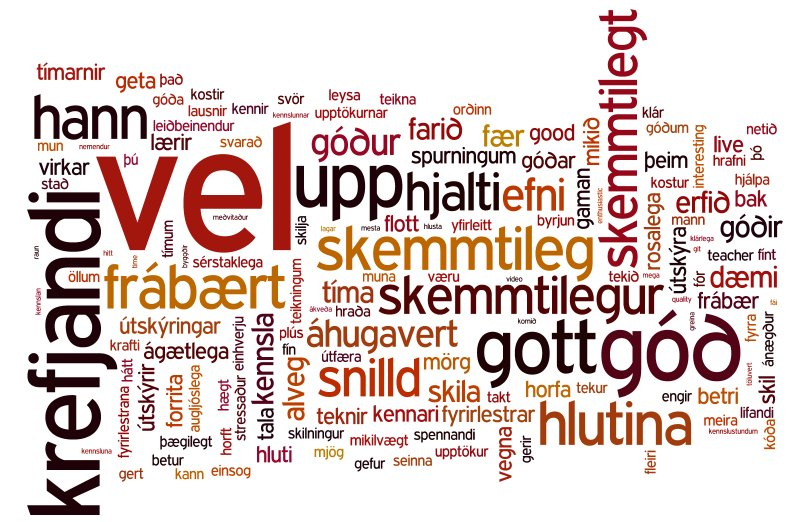
\includegraphics[width=\textwidth]{good-0.jpg}
    \end{figure}
\end{frame}

\begin{frame}{Hva� m�tti b�ta}
    \begin{figure}
        \centering
        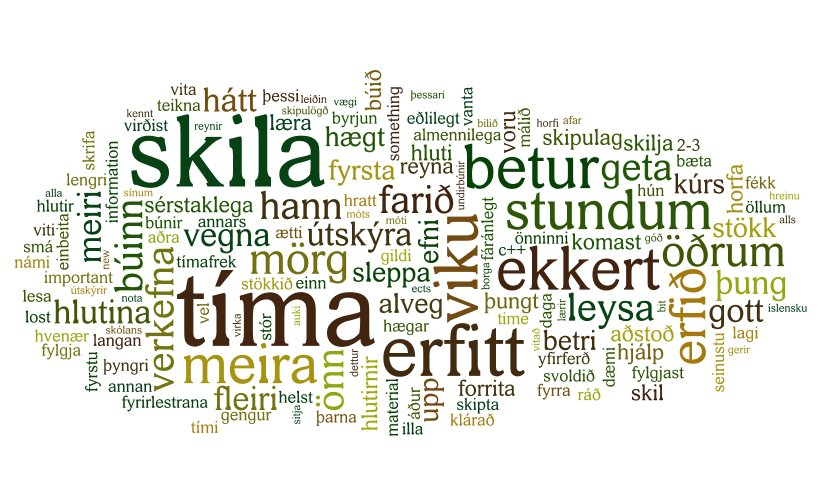
\includegraphics[width=\textwidth]{bad-0.jpg}
    \end{figure}
\end{frame}

\begin{frame}{Helstu atri�i}
    \begin{itemize}
        \item Miki� st�kk �r Forritun
        \item M�rg verkefni
        \item Verkefni skarast
        \item Opnir d�mat�mar
    \end{itemize}
\end{frame}

\begin{frame}{Af hverju verkefni?}
    \begin{quote}
        I hear and I forget. I see and I remember. I do and I understand.
    \end{quote}

    \begin{flushright}
        --- Confucius
    \end{flushright}
\end{frame}

\begin{frame}{Sk�run}
    \begin{itemize}
        \item 7 bestu d�mat�maverkefnin af 11 gilda
        \item A�eins �arf a� gera eitt d�mat�maverkefni samhli�a skilaverkefni
    \end{itemize}
\end{frame}

\begin{frame}{Opnir d�mat�mar}
    \begin{itemize}
        \item Athugasemdum hefur veri� komi� �lei�is til forst��umanns grunnn�ms
    \end{itemize}
\end{frame}


\end{document}

